% Format teze zasnovan je na paketu memoir
% http://tug.ctan.org/macros/latex/contrib/memoir/memman.pdf ili
% http://texdoc.net/texmf-dist/doc/latex/memoir/memman.pdf
% 
% Prilikom zadavanja klase memoir, navedenim opcijama se podešava 
% veličina slova (12pt) i jednostrano štampanje (oneside).
% Ove parametre možete menjati samo ako pravite nezvanične verzije
% mastera za privatnu upotrebu (na primer, u b5 varijanti ima smisla 
% smanjiti 

\documentclass[12pt,oneside]{memoir}

% Paket koji definiše sve specifičnosti mastera Matematičkog fakulteta
\usepackage{matfmaster}
%
% Podrazumevano pismo je ćirilica.
%   Ako koristite pdflatex, a ne xetex, sav latinički tekst na srpskom jeziku
%   treba biti okružen sa \lat{...} ili \begin{latinica}...\end{latinica}.
%
% Opicija [latinica]:
%   ako želite da pišete latiniciom, dodajte opciju "latinica" tj.
%   prethodni paket uključite pomoću: \usepackage[latinica]{matfmaster}.
%   Ako koristite pdflatex, a ne xetex, sav ćirilički tekst treba biti
%   okružen sa \cir{...} ili \begin{cirilica}...\end{cirilica}.
%
% Opcija [biblatex]:
%   ako želite da koristite reference na više jezika i umesto paketa
%   bibtex da koristite BibLaTeX/Biber, dodajte opciju "biblatex" tj.
%   prethodni paket uključite pomoću: \usepackage[biblatex]{matfmaster}
%
% Opcija [b5paper]:
%   ako želite da napravite verziju teze u manjem (b5) formatu, navedite
%   opciju "b5paper", tj. prethodni paket uključite pomoću: 
%   \usepackage[b5paper]{matfmaster}. Tada ima smisla razmisliti o promeni
%   veličine slova (izmenom opcije 12pt na 11pt u \documentclass{memoir}).
%
% Naravno, opcije je moguće kombinovati.
% Npr. \usepackage[b5paper,biblatex]{matfmaster}

% Pomoćni paket koji generiše nasumičan tekst u kojem se javljaju sva slova
% azbuke (nema potrebe koristiti ovo u pravim disertacijama)
\usepackage{pangrami}

% Paket koji obezbeđuje ispravni prikaz ćiriličkih italik slova kada
% se koristi pdflatex. Zakomentarisati ako na sistemu koji koristite ovaj
% paket nije dostupan ili ako ne radi ispravno.
\usepackage{cmsrb}

% Ostali paketi koji se koriste u dokumentu
\usepackage{listings} % listing programskog koda
\usepackage{xcolor}
\lstset{language=C++}

\definecolor{codegreen}{rgb}{0,0.6,0}
\definecolor{codegray}{rgb}{0.5,0.5,0.5}
\definecolor{codered}{rgb}{0.929, 0.173, 0.153}
\definecolor{backcolour}{rgb}{0.95,0.95,0.92}
\definecolor{keywordcolor}{rgb}{0.208, 0.161, 0.988}

\lstdefinestyle{mystyle}{
backgroundcolor=\color{backcolour},   
commentstyle=\color{codegreen},
keywordstyle=\color{keywordcolor},
numberstyle=\tiny\color{codegray},
stringstyle=\color{codered},
basicstyle=\ttfamily\footnotesize,
breakatwhitespace=false,         
breaklines=true,                 
captionpos=b,                    
keepspaces=true,                 
numbers=left,                    
numbersep=5pt,                  
showspaces=false,                
showstringspaces=false,
showtabs=false,                  
tabsize=2
}

\lstset{style=mystyle}

% Datoteka sa literaturom u BibTex tj. BibLaTeX/Biber formatu
\bib{implementacija_tekst_editora_za_pisanje_koda}

% Ime kandidata na srpskom jeziku (u odabranom pismu)
\autor{Бојан Барџић}
% Naslov teze na srpskom jeziku (u odabranom pismu)
\naslov{Имплементација текст едитора за писање кода}
% Godina u kojoj je teza predana komisiji
\godina{2024}
% Ime i afilijacija mentora (u odabranom pismu)
\mentor{др Весна \textsc{Маринковић}, доцент\\ Универзитет у Београду, Математички факултет}
% Ime i afilijacija prvog člana komisije (u odabranom pismu)
\komisijaA{др Милан \textsc{Банковић}, доцент \\ Универзитет у Београду, Математички факултет}
% Ime i afilijacija drugog člana komisije (u odabranom pismu)
\komisijaB{др Иван \textsc{Чукић}, доцент\\ Универзитет у Београду, Математички факултет}
% Ime i afilijacija trećeg člana komisije (opciono)
% \komisijaC{}
% Ime i afilijacija četvrtog člana komisije (opciono)
% \komisijaD{}
% Datum odbrane (obrisati ili iskomentarisati narednu liniju ako datum odbrane nije poznat)
\datumodbrane{15. јануар 2016.}

% Apstrakt na srpskom jeziku (u odabranom pismu)
\apstr{%
\pangrami
}

% Ključne reči na srpskom jeziku (u odabranom pismu)
\kljucnereci{анализа, геометрија, алгебра, логика, рачунарство, астрономија}

\begin{document}
% ==============================================================================
% Uvodni deo teze
\frontmatter
% ==============================================================================
% Naslovna strana
\naslovna
% Strana sa podacima o mentoru i članovima komisije
\komisija
% Strana sa posvetom (u odabranom pismu)
\posveta{Мами, тати и деди}
% Strana sa podacima o disertaciji na srpskom jeziku
\apstrakt
% Sadržaj teze
\tableofcontents*

% ==============================================================================
% Glavni deo teze
\mainmatter
% ==============================================================================

% ------------------------------------------------------------------------------
\chapter{Увод}
% ------------------------------------------------------------------------------

\section{Текст едитори}

\paragraph{}
Текст едитор је програм за измену текстуалних датотека. Најчешћи типови датотека
који се измењују коришћењем ових програма су једноставне текстуалне датотеке, 
датотеке које садржe изворни код, код језика за означавање као и конфигурационе датотеке. 
Неки од најпознатијих оваквих програма су \begin{latinica}\textit{Visual Studio Code}
\end{latinica} \cite{VSC}, \begin{latinica}\textit{Notepad}\end{latinica} \cite{Notepad},
\begin{latinica}\textit{Notepad++}\end{latinica} \cite{Notepad++}, \begin{latinica}\textit{VIM}
\end{latinica} \cite{VIM} и \begin{latinica}\textit{Emacs}\end{latinica} \cite{Emacs}.

\paragraph{}
Постоји више врста текст едитора. Имамо едиторе једноставног текста, где информација
о датотеци предсавља само текст. Док такође постоје и едитори богатог текста, где
информација о датотеци поред текста садржи и неке додатне информације везано за изглед
текста (фонт, величина фонта, боја текста, маргине). Ми ћемо се у овом раду бавити искључиво
едиторима једноставног текста.

\section{Структуре података у текст едиторима}
\paragraph{}
Пошто текст у датотеци можемо посматрати као линеарни низ карактера, 
тако и сваку измену над тим текстом можемо посматрати као додавање текста у
неки део низа или брисање подниза текста. Када бисмо сав текст једне датотеке
које смо отворили чували као један низ карактера, видели бисмо да су горе наведене 
операције јако временски скупе (\(O(n)\), где је \(n\) дужина текста) и да њихово стално 
извршавање над неким великим текстом би имало за последицу изузетну неефикасност текст едитора.
Да би се овај проблем превазишао измишљене су разне структуре података које ове операције
врше ефикасније. Најпознатије овакве структуре су бафер са размацима 
(енг. \begin{latinica}\textit{gap buffer}\end{latinica}), уже (енг. 
\begin{latinica}\textit{rope}\end{latinica}) и табела делова (енг. 
\begin{latinica}\textit{piece table}\end{latinica}).

\subsection{Бафер са размацима}
\paragraph{}
Бафер са размацима (енг. \begin{latinica}\textit{gap buffer}\end{latinica}) је једноставна структура
података која се заснива на једноставној идеји да постоји један линеаран низ чија је средина
"празна", док се са леве и десне стране налази текст. Како ми вршимо измене над неким делом 
текста тако се средина "помера" превлачењем последњег елемента леве стране на почетак десне
или обрнуто. Када се бафер попуни (размак није довољно велики за нову операцију), тада се 
алоцира нови бафер већих димензија, најчешће дупло већи, и у њега се копира текст из старог
бафера.
\paragraph{}
Што се тиче ефикасности ове структуре, у односу на класичан низ, бафер са размацима је доста 
ефикаснији јер немамо нову реалокацију низа при свакој измени. Ефикасност уметања и 
брисања зависи највише од тога колики је размак између индекса на коме желимо да 
извршимо измену текста и леве или десне границе размака. Ако је размак већ на потребној позицији, 
временска сложеност је \(O(1)\). Међутим, ако је размак на једном крају а ми желимо да 
мењамо други крај текста сложеност ће бити \(O(n)\). У просечном случају временска 
сложеност је константна, јер најчешће пишемо карактере један за другим. 
Једина операција која је преостала је алоцирање новог низа, која је линеарне сложености.

\paragraph{}
Ова структура је једноставна за имплементацију и често се користи за једноставне текстуалне
уносе. Познати текст едитор \begin{latinica}\textit{Emacs}\end{latinica} \cite{Emacs} користи 
ову структуру у својој имплементацији. На слици \ref{fig:gap_buffer} приказана је илустрација
рада бафера.

\begin{figure}[!ht]
  \centering
  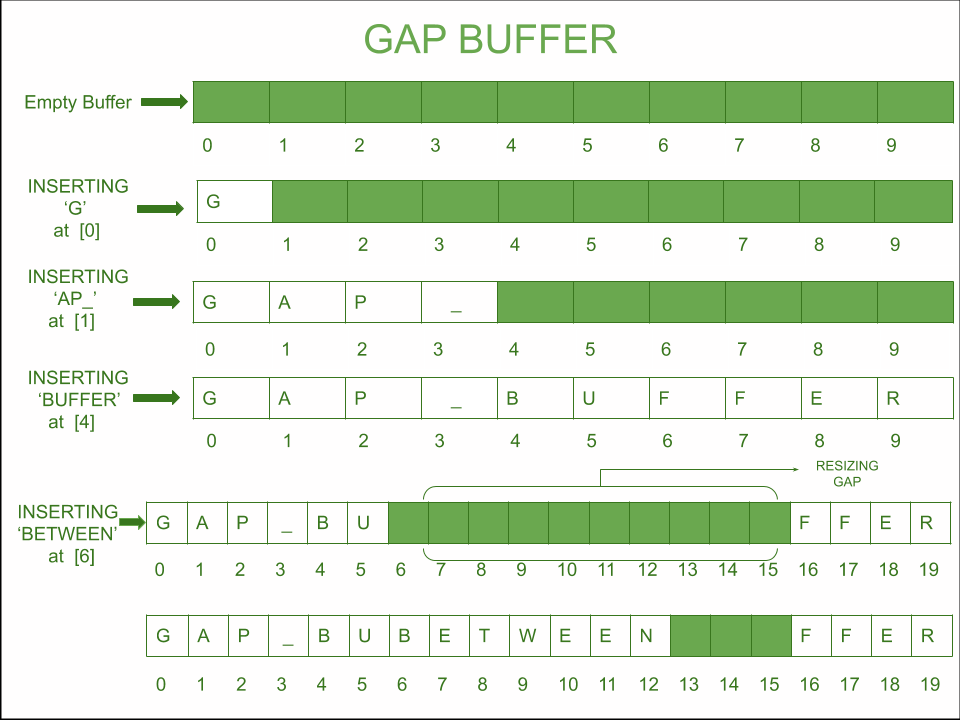
\includegraphics[width=1.0\textwidth]{images/gap_buffer.png}
  \caption{Илустрација бафера са размаком}
  \label{fig:gap_buffer}
\end{figure}

\subsection{Уже}
\paragraph{}
Уже (енг. \begin{latinica}\textit{rope}\end{latinica}) је бинарно стабло где сви чворови који нису
листови садрже број карактера у левом подстаблу тог чвора. У листовима се налазе ниске које 
садрже делове текста. Када се прође кроз од првог листа са лева на десно, добијамо целокупан
текст.

\paragraph{}
Предност ове структуре у односу на обичну ниску је што операције као што су уметање, брисање
и претрага текста не захтевају \(O(n)\) време (где је \(n\) дужина текста), већ \(O(\log{}n)\).
Такође, не морамо да чувамо текст у непрекидном делу меморије, већ се чворови могу налазити на
одвојеним местима.

\paragraph{}
Мане ужета јесу што је то комплексна структура која је склонија баговима, као и што заузима
више меморије него обична ниска (због родитељских чворова који повезују листове).

\subsubsection{Претрага}
\paragraph{}
Претрага карактера на \(i\)-том  индексу се врши тако што пролазимо рекурзивно кроз стабло 
почевши од корена. Ако је индекс мањи од вредности у чвору, настављамо претрагу у левом 
подстаблу. У супротном од \(i\) одузимамо вредност у тренутном чвору и настављамо претрагу у
десном подстаблу. Када наиђемо на лист враћамо \(i\)-ти карактер из ниске која се налази
у чвору. Сложеност операције је иста као код претраге бинарног стабла, а то је \(O(\log{}n)\).
Пример претраге дат је на слици \ref{fig:rope_search}.

\begin{figure}
  \centering
  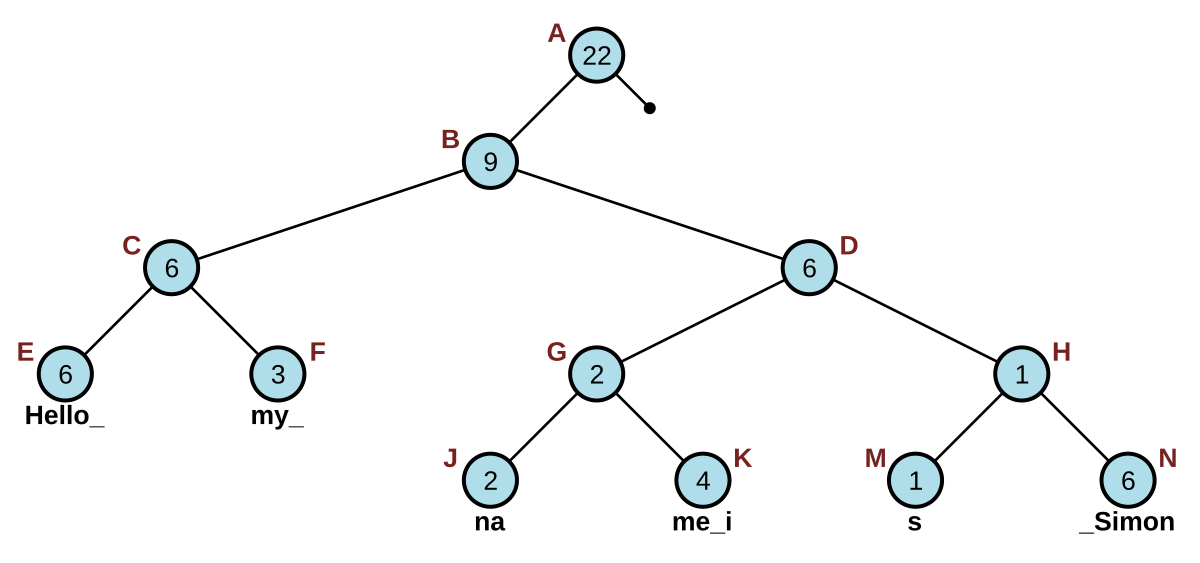
\includegraphics[width=0.8\textwidth]{images/rope_search.png}
  \caption{Претрага помоћу ужета}
  \label{fig:rope_search}
\end{figure}

\subsubsection{Конкатенација}
\paragraph{}
Конкатенација два ужета, \(r_1\) и \(r_2\), се врши тако што направимо нови родитељски чвор
чије ће лево дете бити корен од \(r_1\), а десно корен од  \(r_2\). Вредност новог чвора ће
бити сума дужина ниски у свим листовима \(r_1\). Да бисмо израчунали вредност новог корена
морамо да прођемо кроз све листове десног подстабла \(r_1\), тако да је сложеност ове 
операције \(O(\log{}n)\). Пример конкатенације можемо видети на слици \ref{fig:rope_concat}

\begin{figure}
  \centering
  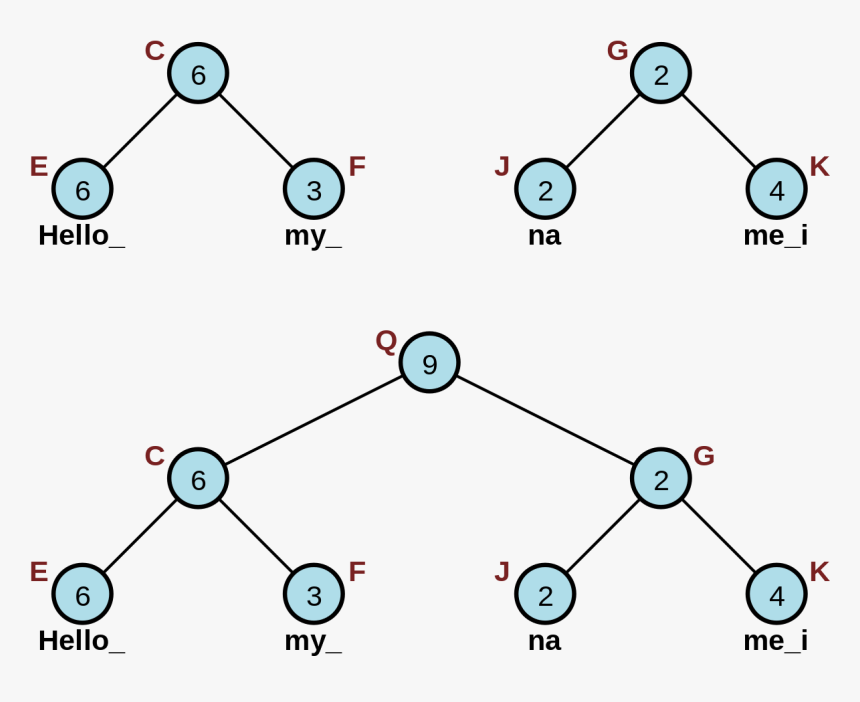
\includegraphics[width=0.8\textwidth]{images/rope_concat.png}
  \caption{Конкатенација два ужета}
  \label{fig:rope_concat}
\end{figure}

\subsubsection{Дељење}
\paragraph{}
Дељење ниске \(s\) по индексу \(i\) на две ниске, \(s_1\) и \(s_2\),
где \(s_1\) садржи карактере од почетка  \(s\) до \(i\)-тог индекса (укључујући и карактер на 
\(i\)-том индексу), а \(s_2\) садржи карактере десно од \(i\)-тог индекса па до краја ниске,
се врши на следећи начин.

\paragraph{}
Налазимо \(i\)-ти карактер, ако је то последњи карактер ниске у листу онда не радимо ништа.
У супротном делимо лист на два нова листа, где је \(i\)-ти карактер последњи карактер ниске
левог листа. Лист где је \(i\)-ти карактер последњи у нисци ћемо означити са \(d\). Сада
листове делимо у две групе \(l_1\)  и \(l_2\). У \(l_1\) се налазе листови лево од \(d\) као и сам \(d\), док се у \(l_2\) налазе листови десно од \(d\). Листове из \(l_2\) одвајамо од 
главног ужета и затим их конкатенирамо заједно. Алгоритам се завршава тако што балансирамо 
два новодобијена ужета. Сложеност је иста као код претходних операција. На слици
\ref{fig:ropе_split} можемо видети пример дељења.

\begin{figure}
  \centering
  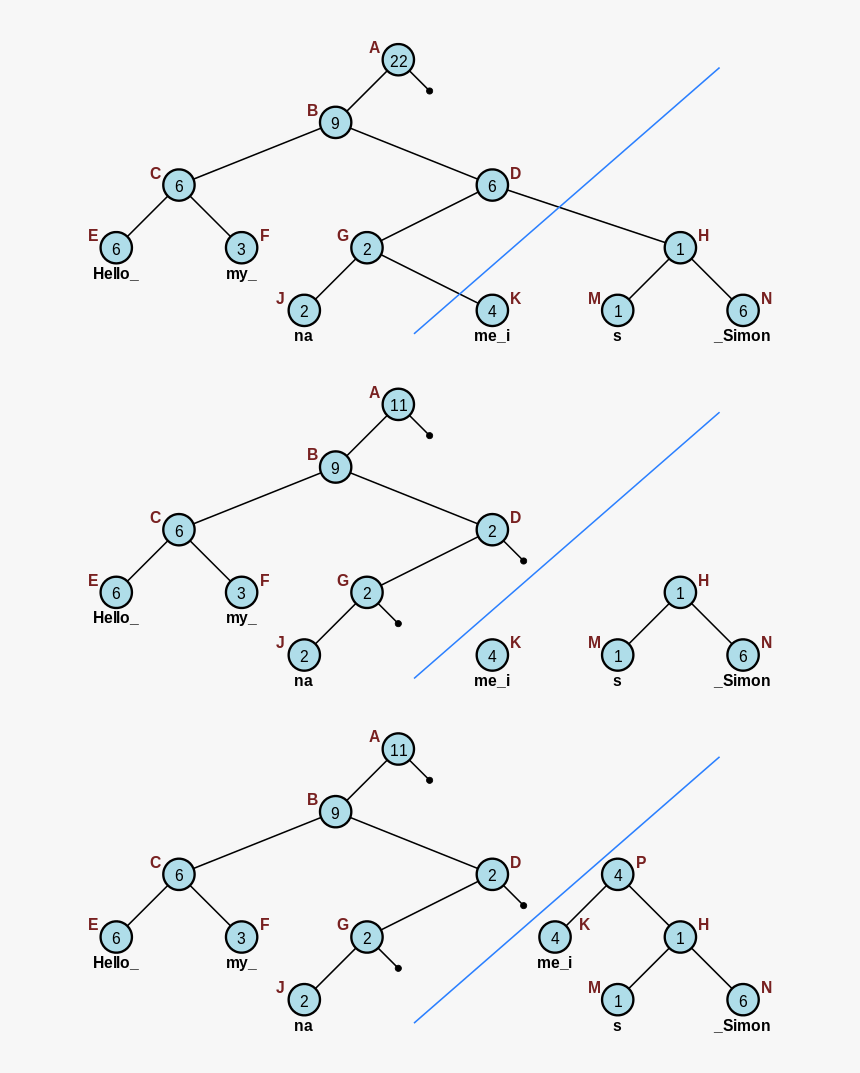
\includegraphics[width=1.0\textwidth]{images/rope_split.png}
  \caption{Дељење ужета}
  \label{fig:ropе_split}
\end{figure} 

\subsubsection{Уметање}
\paragraph{}
Ако желимо да уметнемо неку ниску \(s\) y уже \(r\) на индексу \(i\), довољно је да искористимо претходно дефинисане операције дељења и конкатенације. Прво поделимо уже \(r\) по индексу \(i\)
и добијамо два ужета \(r_1\) и \(r_2\), затим на \(r_1\) конкатенирамо ниску \(s\) и добијемо
ново уже \(r_3\). И на крају конкатенирамо ужад \(r_3\) и \(r_2\). Ова операција се састоји
од три операције сложености \(O(\log{}n)\), тако да је њена сложеност \(O(\log{}n)\).

\subsubsection{Брисање}
\paragraph{}
Уколико желимо да обришемо подниску која почиње на \(i\)-том карактеру, а завршава се на
\((i+l)\)-том каркатеру, онда то можемо урадити у три корака. Прво извршимо дељење по индексу 
\(i\) на \(r_1\) и \(r_2\), затим десну \(r_2\) поделимо по \(l\)-том индексу на \(r_3\)
и \(r_4\). Последњи корак је конкатенирање \(r_1\) и \(r_4\). Из истих разлога као код
уметања, сложеност операције је \(O(\log{}n)\).

\subsection{Табела делова}
\paragraph{}
Табела делова (енг. \begin{latinica}\textit{piece table}\end{latinica}) је структура података
која се састоји од два бафера у којима се налази текст и повезане листе чворова који показују
на текст у баферу. Овај рад је имплементиран помоћу ове структуре података, тако да ћемо проћи
детаљније кроз опис ове структуре него код претходне две.

\paragraph{}
У први бафер се учитава текст који се већ налазио у датотеци коју смо
отворили и тај бафер се назива оригинални бафер (енг. \begin{latinica}\textit{original buffer}\end{latinica}). Од тренутка после учитавања текста из датотеке па надаље он остаје непромењен. 

\paragraph{}
У други бафер додајемо текст који ми уписујемо током времена, овај бафер се
назива бафер за додавање (енг. \begin{latinica}\textit{add buffer}\end{latinica}). Сваки пут
када додајемо текст, он се додаје на његов крај. Важно је напоменути да када бришемо
текст, он се не брише из бафера за додавање, већ остаје у њему. На овај начин немамо потребу
да икада померамо текст који се већ налази унутар бафера.

\paragraph{}
Али како бисмо онда уредили текст да се испише у правилном редоследу? То се постиже
коришћењем двоструко повезане листе (енг. \begin{latinica}\textit{doubly linked list}
\end{latinica}) чији су елементи тзв. дескриптори делова (енг. \begin{latinica}
\textit{piece descriptors}\end{latinica}). Сваки дескриптор садржи информацију о томе на који од
два бафера показује, на којем индексу бафера почиње текст и колика је дужина тог текста. 
Целокупан текст се добија пролажењем кроз повезану листу и надовезивањем свих делова текста, 
по чему је и структура добила име. Следећи код приказује чланске променљиве класе \begin{latinica}
\textit{PieceDescriptor}\end{latinica} у имплементацији рада.

\begin{lstlisting}
class PieceDescriptor {
// ...
private:
    SourceType m_source;
    size_t m_start;
    size_t m_length;
};
\end{lstlisting}

\paragraph{}
Предност ове структуре је што можемо једноставним операцијама, уметањем и брисањем чворова из
повезане листе, да ефикасно вршимо измене текста. Мана је потенцијално велико меморијско заузеће
бафера за додавање као и фрагментација на доста веома малих "делова", што би чинило претрагу
кроз листу мање ефикасном.

\subsubsection{Уношење текста}
\paragraph{}
Ако желимо да додамо неки текст дужине \(d\) у нашу табелу делова на индексу \(i\) прво ћемо
размотрити два специјалана случаја за индекс \(i\).

\begin{enumerate}
	\item \(i=0\): У овом случају само додајемо нови дескриптор на почетак низа.
	\item \(i=n\), где је \(n\) дужина укупног текста: У овом случају додајемо нови дексриптор 
	на крај низа.
\end{enumerate}

За све остале случајеве ћемо проћи кроз листу с лева на десно. Нека је дужина \(ј\)-тог
дескриптора једнака \(d_j\) и нека је сума дужина свих дескриптора пре \(ј\)-тог једнака 
\(s_j\). Када буде важио услов \(s_j + d_j \geq i\) онда разликујемо два случаја:

\begin{enumerate}
	\item \(s_j + d_j = i\): У овом случају убацујемо нови дескриптор испред тренутног на ком се
	налазимо.
	\item \(s_j + d_j > i\): У овом случају делимо тренутни дескриптор на два тако
	да леви садржи \(i - s_j\) карактера оригиналног дескриптора а десни остале.
	Нови дескриптор умећемо између левог и десног.
\end{enumerate}

\subsubsection{Брисање}
\paragraph{}
Брисање неког дела текста који се налзи у опсегу \([b, e)\) се врши на аналоган начин.
Пролазимо кроз повезану листу све док не буде важио услов \(s_j + d_j \geq b\). Сада пролазимо
кроз све дескрипторе који садрже текст из опсега \([s_k, s_k+d_k)\) и имају пресек са \([b, e)\)
и ажурирамо их по следећим правилима:

\begin{enumerate}
	\item Ако је пресек суфикс опсега \([s_k, s_k+d_k)\) дужине \(d_p\), онда одузимамо суфикс 
	од дескриптора тако што му смањујемо дужину за \(d_p\).
	
	\item Ako je пресек префикс опсега \([s_k, s_k+d_k)\) дужине \(d_p\), онда одузимамо префикс
	 од дескриптора тако што померамо почетак у десно и смањујемо дужину за \(d_p\).
	 
	\item Ако је пресек цео опсег \([s_k, s_k+d_k)\), бришемо цео дескриптор.
	 
	\item Ако је \([b, e)\) садржан у \([s_k, s_k+d_k)\) и није ни префикс ни суфикс опсега,
	онда дескриптор делимо на два нова, где први садржи опсег \([s_k, b)\), а други 
	\([e, s_k+d_k)\).
\end{enumerate}



% ------------------------------------------------------------------------------
\chapter{Разрада}
\label{chp:razrada}
% ------------------------------------------------------------------------------

\pangrami

\pangrami

% ------------------------------------------------------------------------------
\chapter{Закључак}
% ------------------------------------------------------------------------------
\pangrami

\pangrami

% ------------------------------------------------------------------------------
% Literatura
% ------------------------------------------------------------------------------
\literatura

% ==============================================================================
% Završni deo teze i prilozi
\backmatter
% ==============================================================================

% ------------------------------------------------------------------------------
% Biografija kandidata
\begin{biografija}
\textbf{Вук Стефановић Караџић} (\emph{Тршић, 26. октобар/6. новембар
  1787. — Беч, 7. фебруар 1864.}) био је српски филолог, реформатор
српског језика, сакупљач народних умотворина и писац првог речника
српског језика.  Вук је најзначајнија личност српске књижевности прве
половине XIX века. Стекао је и неколико почасних доктората.
Учествовао је у Првом српском устанку као писар и чиновник у
Неготинској крајини, а након слома устанка преселио се у Беч,
1813. године. Ту је упознао Јернеја Копитара, цензора словенских
књига, на чији је подстицај кренуо у прикупљање српских народних
песама, реформу ћирилице и борбу за увођење народног језика у српску
књижевност. Вуковим реформама у српски језик је уведен фонетски
правопис, а српски језик је потиснуо славеносрпски језик који је у то
време био језик образованих људи. Тако се као најважније године Вукове
реформе истичу 1818., 1836., 1839., 1847. и 1852.
\end{biografija}
% ------------------------------------------------------------------------------

\end{document} 